\chapter{}
\label{chp:appA}

\section{Example Discussion}
Figure \ref{fig:dsbo-example} shows a 2-dimensional search space example for which \textit{Distributed SafeOpt} is applied for optimization. 
$H1$ nad $H2$ are two dimensions of search space with bounds $(-8, 8)$ and $(-8, 8)$ respectively. 
Here we divide each dimension into four subspaces, so total $2^4=16$ hyperspaces are possible, i.e., the combination of subspace-2 of $H1$ and subspace-3 of $H2$ is hyperspace-11. 
The point in the safe seed $S_0$ belongs to hyperspace-10. 
Used green and red colors to represent the algorithm's safe and unsafe evaluations, respectively. 
Figure \ref{fig:dsbo-example-a} shows an initial state of the optimization, where a safe seed in hyperspace-10 is deployed into node-0. 
Figure \ref{fig:dsbo-example-b} shows a newly sampled safe point in hyperspace-15, so the search space is split between hyperspace-10 and hyperspace-15 as shown in figure \ref{fig:dsbo-example-c} with different colors.
So the first search space has bounds $[(-8,4), (-8,8)]$ with a safe seed in hyperspace-10. Similarly, the second search space has bounds $[(4,8),(-8,8)]$ with a safe seed in hyperspace-15.
This second search space is deployed into a new node (node-1), whereas the first search space is redeployed in the same node (node-0).

We have two optimization processes at two different nodes, independently sample the next points of interest, and follow the algorithm to split the search space.
One thing to notice in node-1 (see figure \ref{fig:dsbo-example-d} right side search space) the next point sampled is unsafe, so the search space splitting will not happen until a safe point in some other hyperspace is found.
Once the search space bounds reduce to the single hyperspace bounds like hyperspace-15 in figure \ref{fig:dsbo-example-f}, we consider it as a leaf node, and no further splitting of search space will happen.\\


\begin{figure}
	\centering
	\begin{subfigure}{0.45\textwidth}
		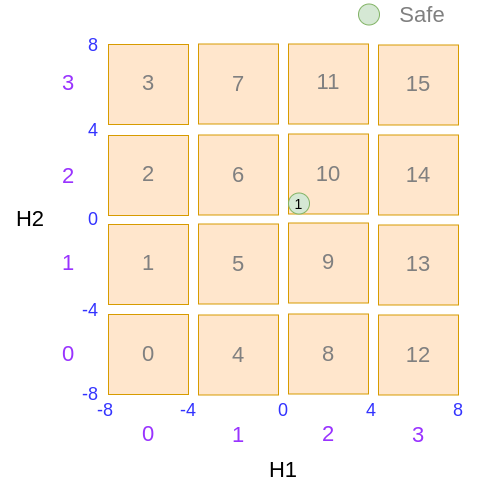
\includegraphics[width=0.8\textwidth]{figures/draw/a.png}
		\caption{}
		\label{fig:dsbo-example-a}
	\end{subfigure}
	%	\hfill
	\begin{subfigure}{0.45\textwidth}
		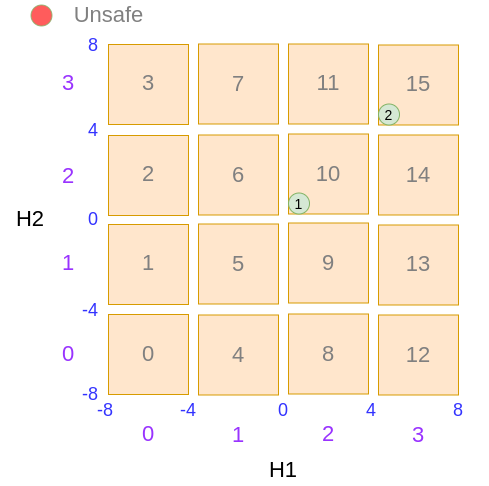
\includegraphics[width=0.8\textwidth]{figures/draw/b.png}
		\caption{}
		\label{fig:dsbo-example-b}
	\end{subfigure}
	\begin{subfigure}{0.45\textwidth}
		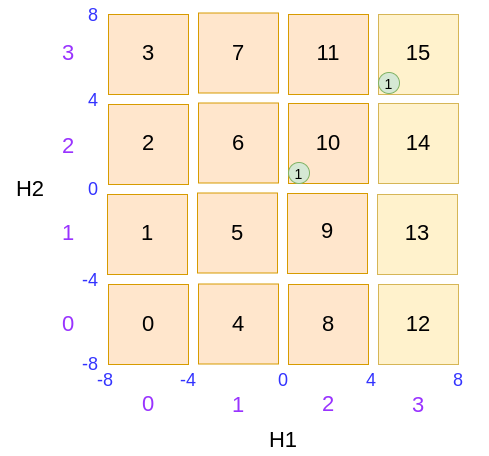
\includegraphics[width=0.8\textwidth]{figures/draw/c.png}
		\caption{}
		\label{fig:dsbo-example-c}
	\end{subfigure}
	\begin{subfigure}{0.45\textwidth}
		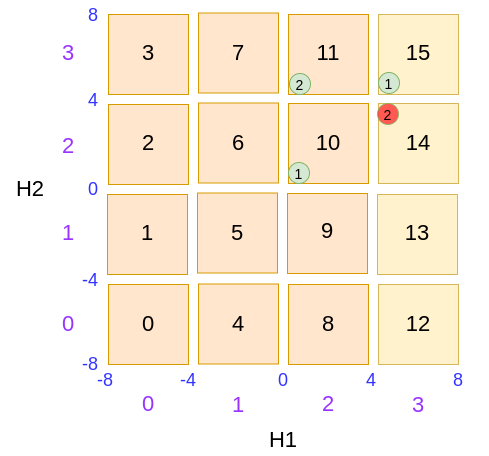
\includegraphics[width=0.8\textwidth]{figures/draw/d.png}
		\caption{}
		\label{fig:dsbo-example-d}
	\end{subfigure}
	\begin{subfigure}{0.45\textwidth}
		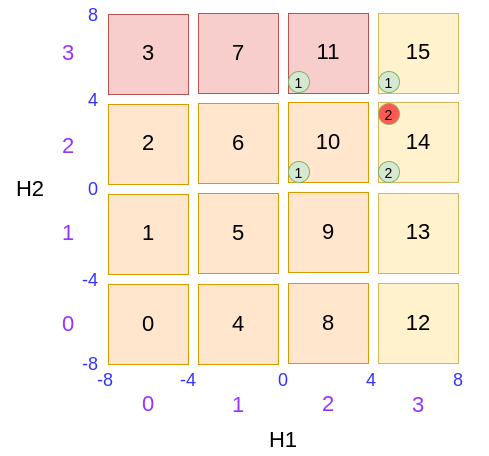
\includegraphics[width=0.8\textwidth]{figures/draw/e.png}
		\caption{}
		\label{fig:dsbo-example-e}
	\end{subfigure}
	%	\hfill
	\begin{subfigure}{0.45\textwidth}
		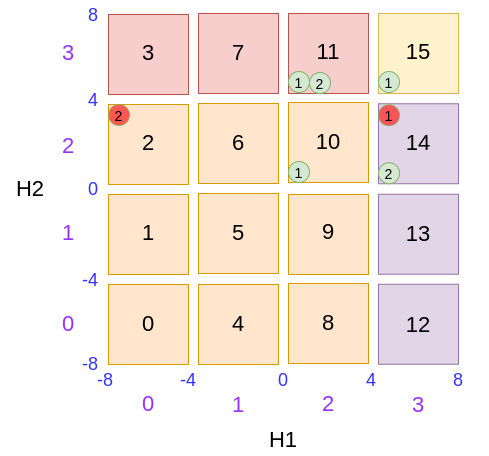
\includegraphics[width=0.8\textwidth]{figures/draw/f.png}
		\caption{}
		\label{fig:dsbo-example-f}
	\end{subfigure}
	\begin{subfigure}{0.45\textwidth}
		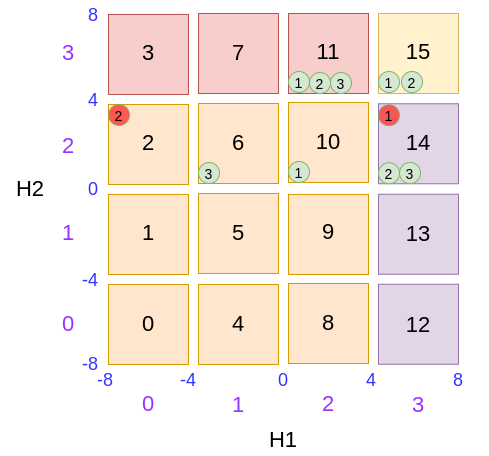
\includegraphics[width=0.8\textwidth]{figures/draw/g.png}
		\caption{}
		\label{fig:dsbo-example-g}
	\end{subfigure}
	\begin{subfigure}{0.45\textwidth}
		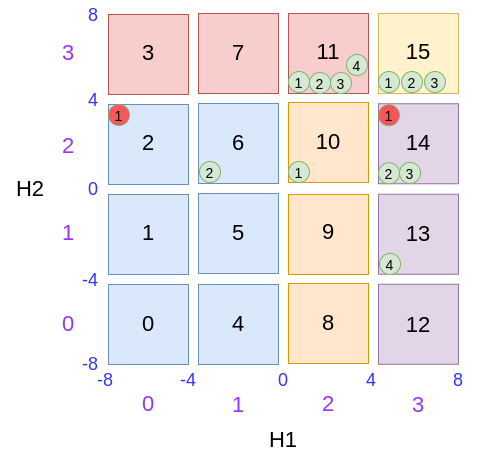
\includegraphics[width=0.8\textwidth]{figures/draw/h.png}
		\caption{}
		\label{fig:dsbo-example-h}
	\end{subfigure}
	\caption{Illustration of algorithm for a 2-dimensional search space example}
	\label{fig:dsbo-example}
\end{figure}

